%-------------------------------------------------------------------------------
%                                PREAMBLE
%-------------------------------------------------------------------------------
\documentclass[usenames,dvipsnames,svgnames,10pt,aspectratio=169]{beamer}
%
\usefonttheme{professionalfonts}
% This theme uses TIKZ: compile twice with PDFLaTeX or LuaLaTeX.
%
%  Options:
%  - [clean]:    clean slides, i.e. logos and footbar are removed
%  - [kth]:      footbar style inspierd to the official KTH template
%  - [nicewave]: a different style of wave is used (not approved by FLOW)
%
\usetheme{flow}

\usepackage{hyperref,graphicx,lmodern}
\usepackage[utf8]{inputenc}
\usepackage{media9}
\usepackage{xcolor}
\usepackage{stmaryrd}
\usepackage{nicefrac}
\usepackage{multimedia}
\usepackage{multicol}
\usepackage{upgreek}
\usepackage[]{bm}
\usepackage[]{url}
\usepackage[]{animate}

\graphicspath{{imgs/}}
\setbeamertemplate{blocks}[rounded][shadow=true]


%-------------------------------------------------------------------------------
%                                TITLE PAGE
%-------------------------------------------------------------------------------
\title[Nonlinear physics] % Short title used in footline
{
	Physique non-lin\'eaire, syst\`emes \\ dynamiques et th\'eorie du chaos
}

\author[J.-Ch.~Loiseau] % Presenting author in short form used in footline
{
	\underline{Jean-Christophe Loiseau}
}
% - Give the names in the same order as the appear in the paper.
% - Underline the presenting author.

\institute[unused]
{
	\url{jean-christophe.loiseau@ensam.eu} \\
	Laboratoire DynFluid \\
	Arts et M\'etiers ParisTech, France.
}
% Keep it simple, no one is interested in your street address.

% University logo(s)
\logot{
\includegraphics[width=.128\paperwidth]{DynFluid_logo}}  % Top logo
\logob{
\includegraphics[width=0.128\paperwidth]{ENSAM_logo}} % Bottom logo
% \logoc[{
\includegraphics[width=.128\paperwidth]{limsi}}]{
\includegraphics[width=.128\paperwidth]{limsi}} % Corner logo
%
% Cover image: \cvrimg{x position}{y position}{cover image}
\cvrimg{.77}{.8}{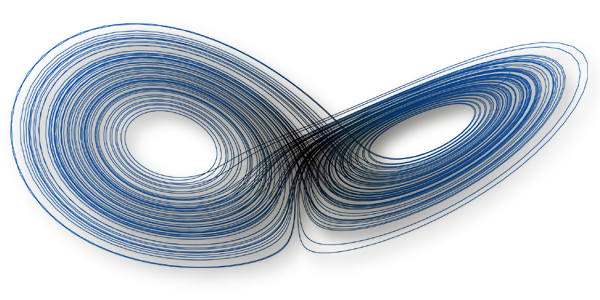
\includegraphics[width=.4\paperwidth]{cover.png}}

\date[unused]{Physique non-lin\'eaire -- 2018-2019}

\begin{document}

\titleframe % Print the title as the first slide

%-------------------------------------------------------------------------------
%                           PRESENTATION SLIDES
%-------------------------------------------------------------------------------

\begin{frame}[t, c]{Remarques générales}{}
	\begin{itemize}
		\item Les cours ont lieu chaque \textbf{\alert{Mardi}} et \textbf{\alert{Jeudi}}, de 15h30 à 17h30 jusqu'à fin février.

		\bigskip

		\item L'évaluation se fera en deux parties:
		\begin{itemize}
			\item[$\hookrightarrow$] Un devoir sur table de 2h fin février.
			\item[$\hookrightarrow$] Un projet alliant mathématiques et simulations numériques.
		\end{itemize}

		\bigskip

		\item Révisez vos cours d'algèbre linéaire si vous n'êtes pas au point.

	\end{itemize}
\end{frame}

\begin{frame}[t, c]{Projet numérique}{}

	\begin{itemize}
		\item Le projet numérique se fera en \alert{\textbf{Python 3.6}} ou \alert{\textbf{Julia}}.

		\bigskip

		\item Vous pouvez télécharger la distribution \alert{\textbf{Anaconda}} sur \url{https://www.anaconda.com/}
		\begin{itemize}
			\item[$\hookrightarrow$] Disponible pour Windows, Mac et Linux.
		\end{itemize}

		\bigskip

		\item De nombreux tutoriels sont disponibles en ligne pour vous familiariser avec Python.
		\begin{itemize}
			\item[$\hookrightarrow$] \url{https://www.codecademy.com/} est un bon endroit pour commencer.
			\item[$\hookrightarrow$] \url{https://github.com/UCIDataScienceInitiative/IntroToJulia} également.
		\end{itemize}

	\end{itemize}

	\vspace{1cm}
\end{frame}

\begin{frame}[t, c]{Quelques références utiles}{Niveau: débutant, lecture vivement conseillée!}
	\begin{itemize}
		\item Ian Stewart, \emph{Dieu joue-t'il au dés?}, Flammarion (2004).
		\bigskip
		\item James Gleick, \emph{La théorie du chaos}, Flammarion (2008).
		\bigskip
		\item Ilya Prigogine, \emph{Les lois du chaos}, Flammarion (2008).
	\end{itemize}

	\vspace{1cm}
\end{frame}

\begin{frame}[t, c]{Quelques références utiles}{Niveau: avancé}
	\begin{itemize}
		\item Y. Pomeau, M. Dubois Gance et P. Bergé, \emph{Des rythmes au chaos}, Odile Jacobi (1994).

		\bigskip

		\item P. Bergé, Y. Pomeau et C. Vidal, \emph{L'order dans le chaos}, Hermann (1998).

		\bigskip

		\item P. Manneville, \emph{Instabilités, chaos et turbulence}, Editions de l'Ecole Polytechnique (2004).
	\end{itemize}

	\vspace{1cm}
\end{frame}


%%%%%
%%%%%
%%%%%     Examples de systèmes dynamiques
%%%%%
%%%%%


\begin{frame}[t, c]{}{}

	\centering

	{\Large \textbf{Qu'est un système dynamique?}}

	\bigskip

	\textgre{\textbf{Quelques exemples}}

	\vspace{-2cm}
\end{frame}

\begin{frame}[t, c]{Quelques exemples...}{Le pendule simple}
	\begin{minipage}{0.38\textwidth}
		\centering
		
\includegraphics[width=.75\textwidth]{tournesol_pendule}
	\end{minipage}%
	\hfill
	\begin{minipage}{0.58\textwidth}
		\begin{itemize}
			\item L'évolution de sa position angulaire $\theta(t)$ au cours du temps est gouvernée par
					\begin{equation}
						\ddot{\theta} + 2k \dot{\theta} + \omega_0^2 \sin(\theta) = 0.
						\notag
					\end{equation}

			\item C'est une équation différentielle ordinaire (EDO) non-linéaire.
			\begin{itemize}
				\item[$\hookrightarrow$] Pas de solution analytique.
			\end{itemize}
		\end{itemize}

		\vspace{1cm}
	\end{minipage}
\end{frame}

\begin{frame}[t, c]{Quelques exemples...}{L'écoulement autour d'un cylindre}
	\begin{minipage}{0.48\textwidth}
		\begin{itemize}
			\item La dynamique de l'écoulement est gouvernée par les équations de Navier-Stokes
			\begin{equation}
				\begin{aligned}
					\displaystyle \frac{\partial {\bm u}}{\partial t} + ({\bm u} \cdot \nabla ) {\bm u} & = - \nabla p + \frac{1}{Re}\nabla^2 {\bm u} + {\bm f}\\
					\nabla \cdot {\bm u} & = 0.
				\end{aligned}
				\notag
			\end{equation}

			\item Ce sont des équations non-linéaires aux dérivées partielles.
			\begin{itemize}
				\item[$\hookrightarrow$] Très peu de solutions analytiques.
			\end{itemize}

		\end{itemize}
	\end{minipage}%
	\hfill
	\begin{minipage}{0.48\textwidth}
		\begin{center}
			\movie[width=\textwidth, autostart, loop]{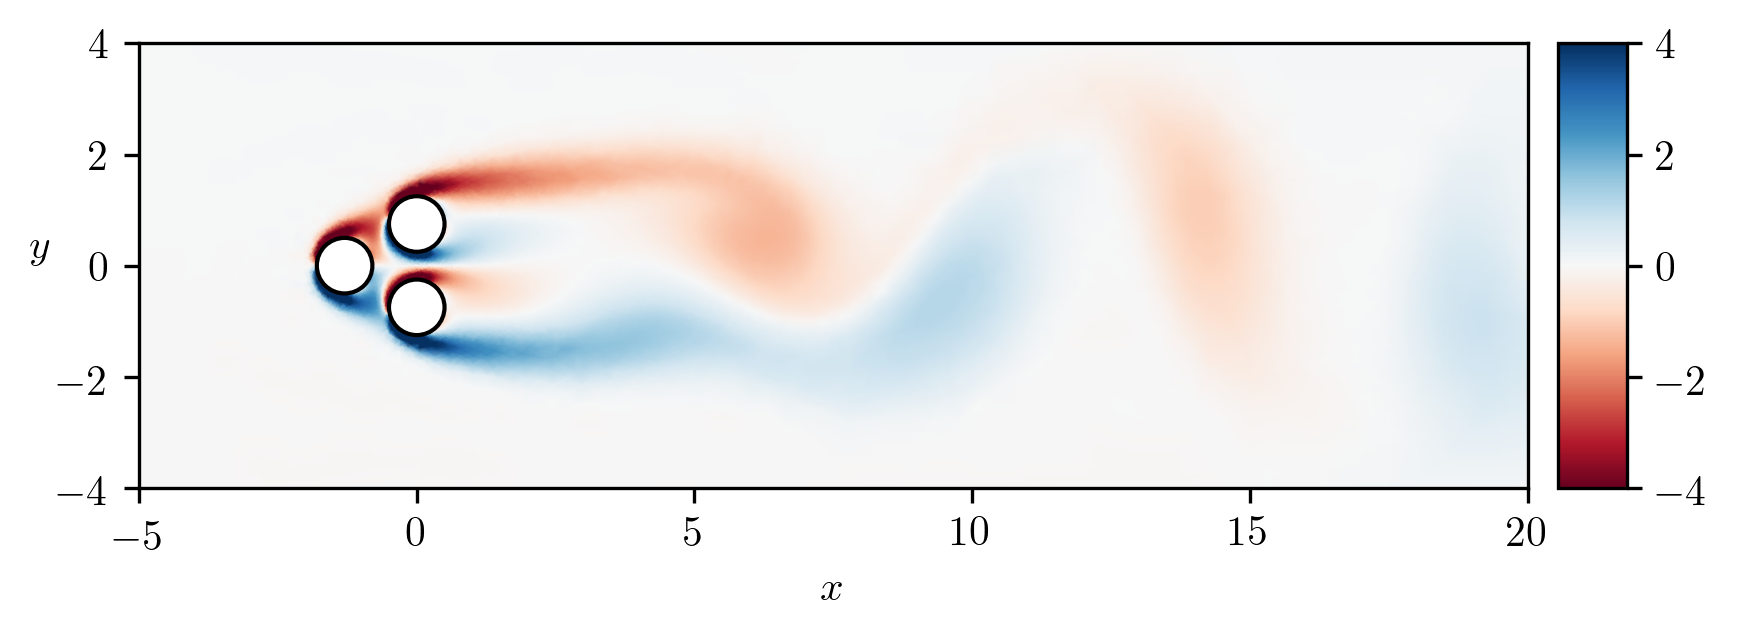
\includegraphics[width=\textwidth]{fluidic_pinball_Re60_snapshot}}{imgs/fluidic_pinball_Re60.mp4}
		\end{center}

		{\small Evolution temporelle du champ de vorticité autour d'un trio de cylindre. Notez que la vitesse de rotation des cylindres n'est pas constante.}
	\end{minipage}
\end{frame}

\begin{frame}[t, c]{Quelques exemples...}{Le modèle de Lotka-Volterra}
	\begin{minipage}{.48\textwidth}
		\centering
		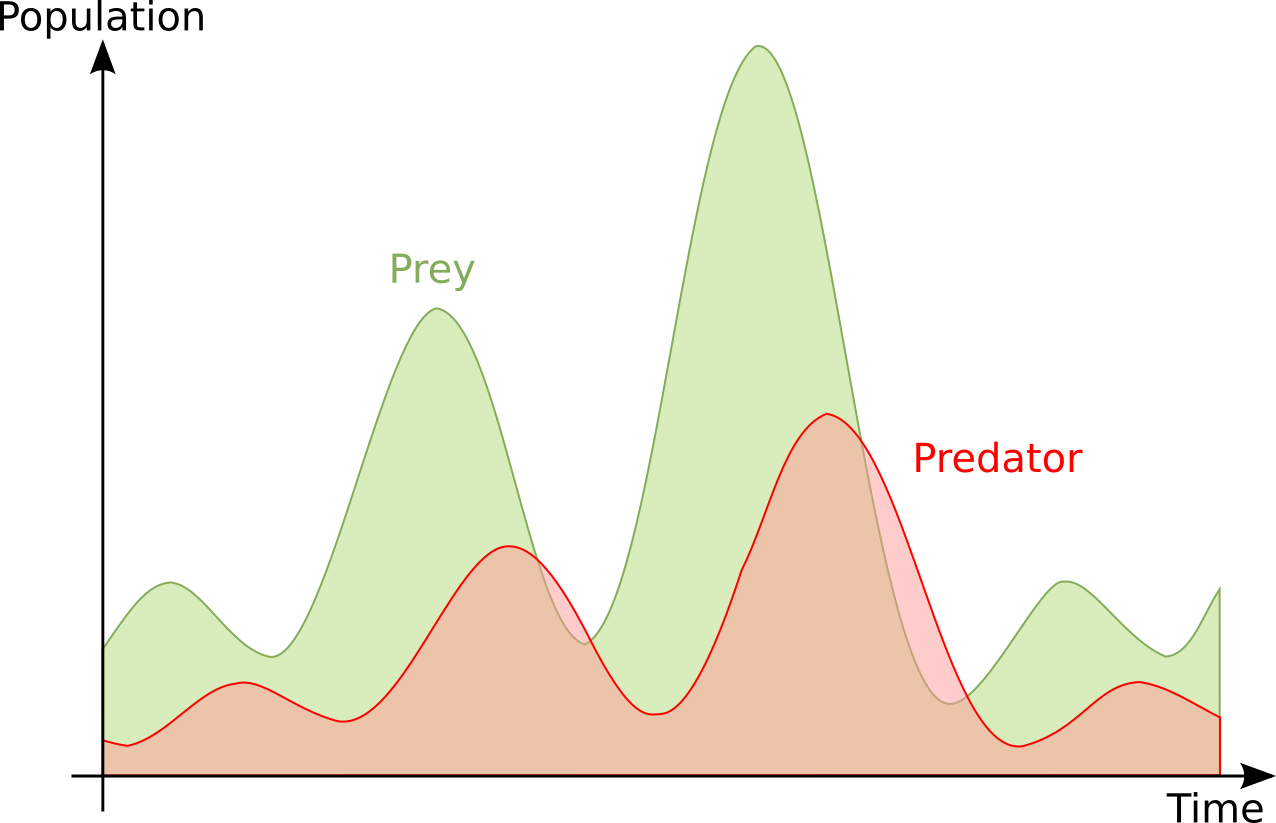
\includegraphics[width=.9\textwidth]{Lotka_Volterra}
	\end{minipage}%
	\hfill
	\begin{minipage}{.48\textwidth}
		\begin{itemize}
			\item L'évolution d'une population de proies et de prédateurs peut être modélisée par
			\begin{equation}
				\begin{aligned}
					\displaystyle \frac{\mathrm{d} x}{\mathrm{d}t} & = \alpha x - \beta xy,\\
					\displaystyle \frac{\mathrm{d} y}{\mathrm{d}t} & = \delta x y - \gamma y.
				\end{aligned}
				\notag
			\end{equation}

			\item C'est un système de deux équations différentielles ordinaires non-linéairement couplées.
		\end{itemize}
	\end{minipage}
\end{frame}

\begin{frame}[t, c]{Quelques exemples...}{Le problème des trois corps}
	\begin{minipage}{.48\textwidth}
		\begin{itemize}
			\item Le problème des trois corps peut être utilisé pour modéliser l'évolution d'un satellite autour de la Terre et de la Lune.
			\bigskip
			\item C'est un système de trois équations différentielles ordinaires non-linéairement couplées.
		\end{itemize}
	\end{minipage}%
	\hfill
	\begin{minipage}{.48\textwidth}
		\centering
		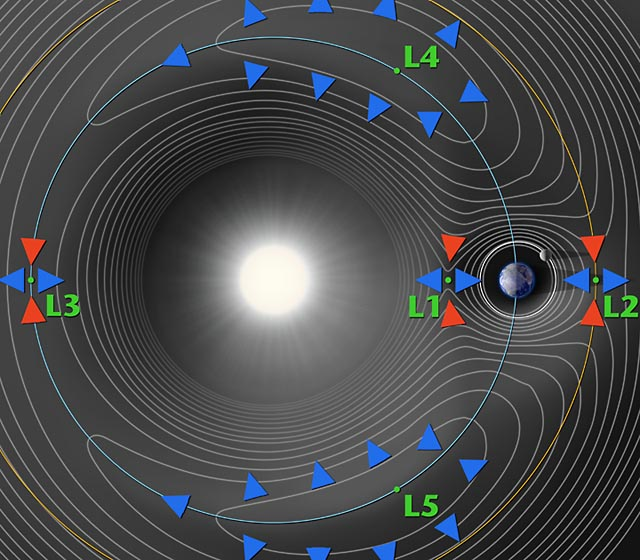
\includegraphics[width=.8\textwidth]{trois_corps}
	\end{minipage}
	\vspace{1cm}
\end{frame}

\begin{frame}[t, c]{Quelques exemples...}{Systèmes dynamiques en temps continu}

	\begin{itemize}
		\item Tous ces systèmes peuvent être écrits sous la forme
		\begin{equation}
			\dot{\bm x} = \bm{f}({\bm x}, \lambda)
			\notag
		\end{equation}
		où ${\bm x}$ est le \emph{vecteur d'état} du système, $\lambda$ un vecteur de \emph{paramètres} et $\bm{f}({\bm x}, \lambda)$ une fonction non-linéaire.

		\bigskip

		\item \`A noter que l'on pré-suppose ici que le temps $t$ est continu.
	\end{itemize}

	\vspace{1cm}
\end{frame}

\begin{frame}[t, c]{Quelques exemples...}{Systèmes dynamiques en temps discret}

	\begin{itemize}
		\item Si l'on a qu'une vue \emph{stroboscopique} du système, sa dynamique peut alors être exprimée de la façon suivante
		\begin{equation}
			{\bm x}^{(n+1)} = \bm{F}({\bm x}^{(n)}, \lambda)
			\notag
		\end{equation}
		où $n$ définie maintenant l'instant discret.

		\bigskip

		\item Ce genre de modèle est appelé un \emph{système dynamique à temps discret}, un \emph{itéré} ou encore une \emph{map}.
	\end{itemize}

		\vspace{1cm}
\end{frame}


%%%%%
%%%%%
%%%%%     Quelques définitions nécessaires pour la suite
%%%%%
%%%%%

\begin{frame}[t, c]{}{}

	\centering

	{\Large \textbf{Comment étudie-t'on un système dynamique?}}

	\bigskip

	\textgre{\textbf{Un petit aperçu de ce qui vous attend...}}

	\vspace{-2cm}
\end{frame}

\begin{frame}[t, c]{Qu'est ce qu'un système linéaire?}{}
	\begin{block}{}
		\centering
		Considérons le système dynamique suivant
		$$ \dot{\bm x} = {\bm f}({\bm x}).$$
		Sous quelle(s) condition(s) est-il \alert{\textbf{linéaire}}?
	\end{block}

	\vspace{1cm}
\end{frame}

\begin{frame}[t, c]{Qu'est ce qu'un système linéaire?}{Quelques définitions...}

	\begin{itemize}
		\item 	Soit ${\bm u}(t)$ et ${\bm v}(t)$ deux solutions du système. Ce dernier est dit \alert{\textbf{linéaire}} si :
			\medskip
			\begin{itemize}
				\item[$\hookrightarrow$] ${\bm w}(t) = \alpha {\bm u}(t) + \beta {\bm v}(t)$ est aussi solution du système,
				\medskip
				\item[$\hookrightarrow$] ${\bm f}(\alpha {\bm u} + \beta {\bm v}) = \alpha {\bm f}({\bm u})  + \beta {\bm f}({\bm v})$,
				\medskip
				\item[$\hookrightarrow$] Il obéît au \alert{\textbf{principe de superposition}}.
			\end{itemize}

		\medskip

		\item Le système peut alors être écrit sous la forme
			$$ \dot{\bm x} = {\bm A}{\bm x},$$
			où ${\bm A}$ est un opérateur linéaire.

		\medskip

		\item Sa solution est alors
		$${\bm x}(t) = e^{{\bm A}t} {\bm x}_0.$$
	\end{itemize}

	\vspace{1cm}
\end{frame}

\begin{frame}[t, c]{Qu'est ce qu'un système linéaire?}{Exemple: l'oscillateur harmonique}
	\begin{minipage}{.48\textwidth}
		\begin{itemize}
			\item La dynamique d'un oscillateur harmonique est gouvernée par
			$$\ddot{x} = - \omega_0^2 x.$$

			\medskip

			\item En posant $y = \dot{x}$, on obtient alors
			$$\displaystyle \frac{\mathrm{d}}{\mathrm{d}t} \begin{bmatrix} x \\ y \end{bmatrix} = \begin{bmatrix} 0 & 1 \\ -\omega_0^2 & 0 \end{bmatrix} \begin{bmatrix} x \\ y \end{bmatrix}.$$
		\end{itemize}
	\end{minipage}%
	\hfill
	\begin{minipage}{.48\textwidth}
		\centering
		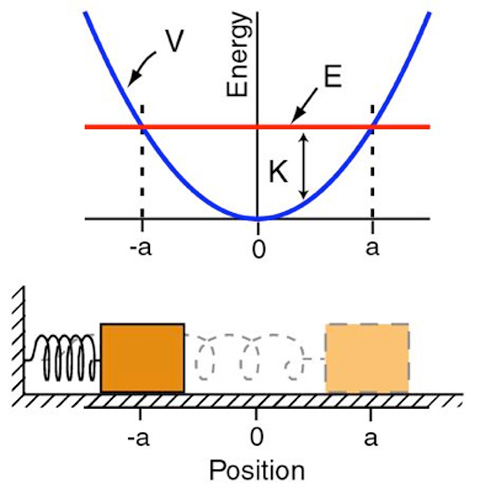
\includegraphics[width=.8\textwidth]{harmonic_oscillator}
	\end{minipage}

	\vspace{1cm}
\end{frame}

\begin{frame}[t, c]{}{}
	\begin{block}{\centering \textbf{Attention!}}
		Si les sytèmes linéaires sont apparus si fréquemment tout au long de vos études, c'est uniquement parce qu'ils sont plus faciles à étudier! Beaucoup de systèmes linéaires en apparance ne sont en réalité qu'une approximation d'un système non-linéaire plus complexe.
	\end{block}
\end{frame}

\begin{frame}[t, c]{Qu'est ce qu'un système non-linéaire?}{}
	\begin{block}{\centering \textbf{Définition}}
		\centering
		C'est un système qui n'est pas linéaire.
	\end{block}

	\vspace{1cm}
\end{frame}

\begin{frame}[t, c]{Qu'est ce qu'un système non-linéaire?}{Quelques exemples}
	\begin{itemize}
		\item L'oscillateur de \emph{van der Pol}
		$$\ddot{x} - \epsilon (1 - x^2) \dot{x} + \omega_0^2 x = 0$$
		permet de modéliser le potentiel d'action des neurones ou d'étudier l'intéraction des plaques au niveau d'une faille de subduction.

		\medskip

		\item L'émission de photons par un laser est modélisée par
		$$\dot{n} = gn ( N_0 - an) - kn$$
		où $g$ est le gain du laser, $k$ décrit le taux de pertes et $N(t) = N_0 - an$ est le nombre d'atomes excités.

	\end{itemize}

	\vspace{1cm}
\end{frame}

\begin{frame}[t, c]{}{}

	\centering

	{\Large \textbf{Illustration}}

	\bigskip

	\textgre{\textbf{Le pendule simple}}

	\vspace{-2cm}
\end{frame}

\begin{frame}[t, c]{Le pendule simple}{}
	\begin{minipage}{.48\textwidth}
		\begin{itemize}
			\item La dynamique angulaire d'un pendule simple est gouvernée par
			$$\ddot{\theta} = -2k \dot{\theta} -\omega_0^2 \sin(\theta).$$

			\bigskip

			\item En posant $x = \theta$ et $y = \dot{\theta}$, on obtient alors
			\begin{equation}
				\begin{aligned}
					\dot{x} & = y \\
					\dot{y} & = -2k y -\omega_0^2 \sin(x).
				\end{aligned}
				\notag
			\end{equation}
		\end{itemize}
	\end{minipage}%
	\hfill
	\begin{minipage}{.48\textwidth}
		\centering
		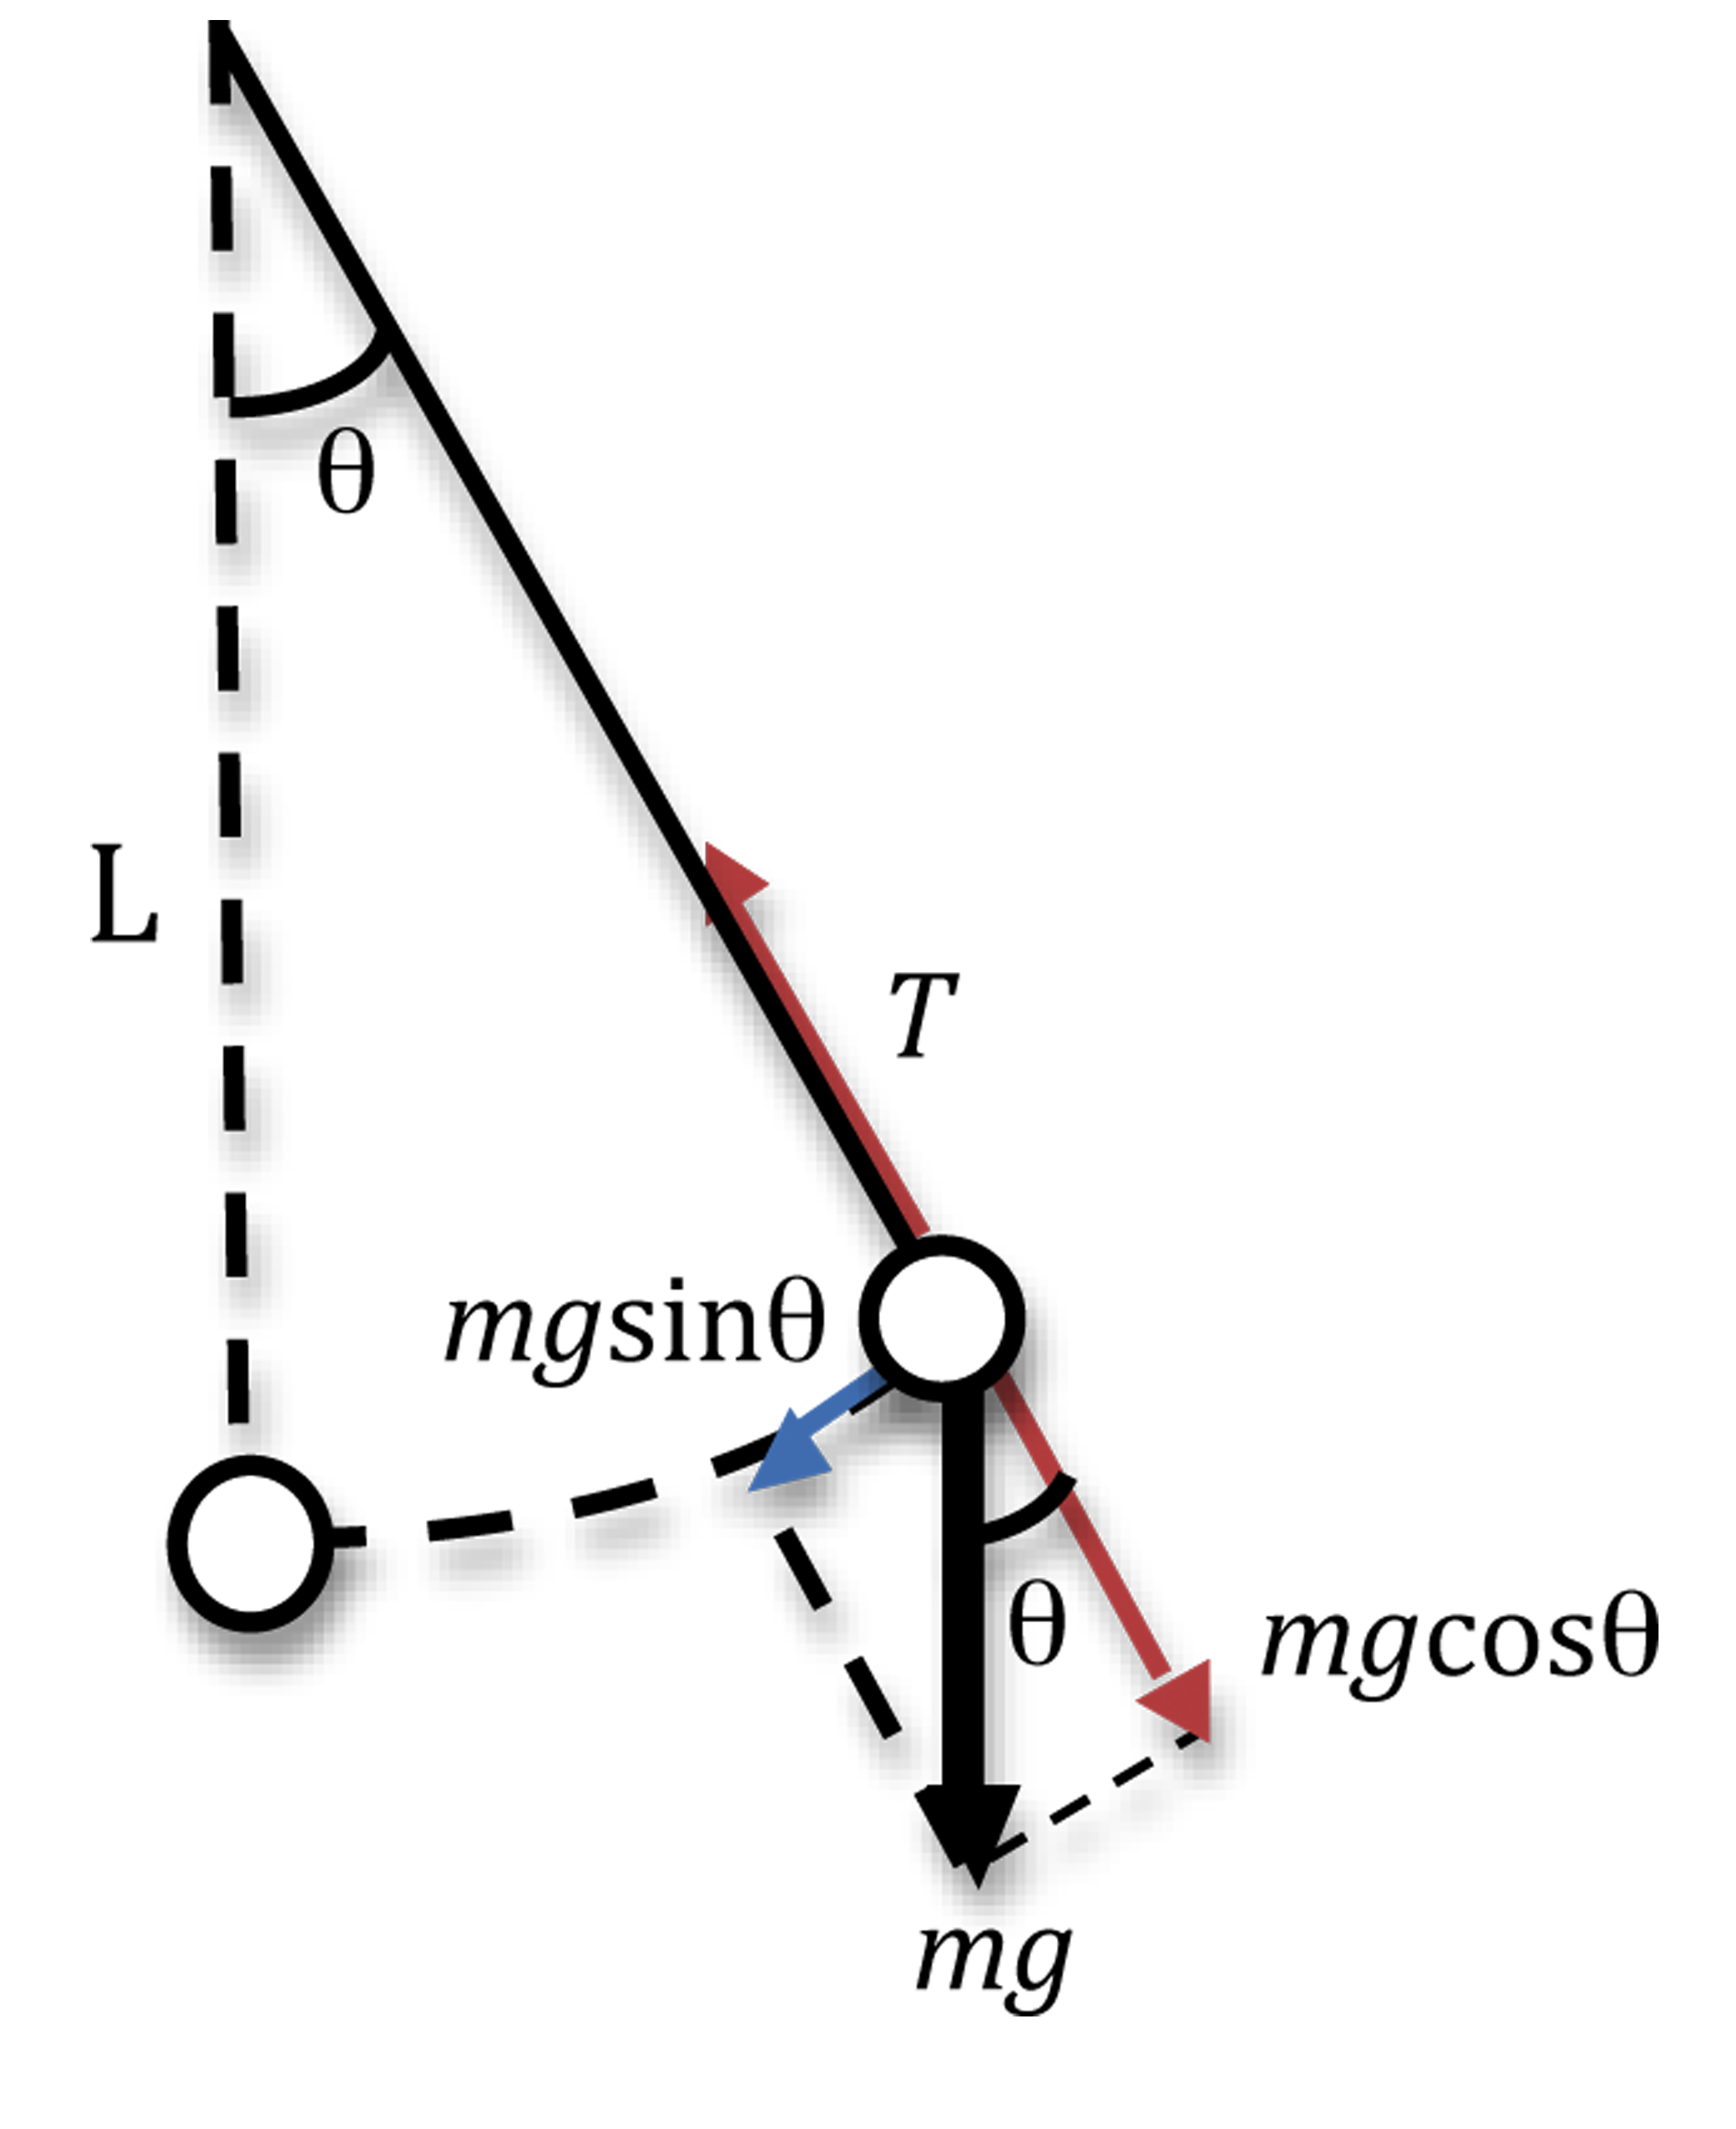
\includegraphics[width=.75\textwidth]{pendulum_sketch}
	\end{minipage}

	\vspace{0.5cm}
\end{frame}

\begin{frame}[t, c]{Le pendule simple}{Plan de phase}
	\centering
	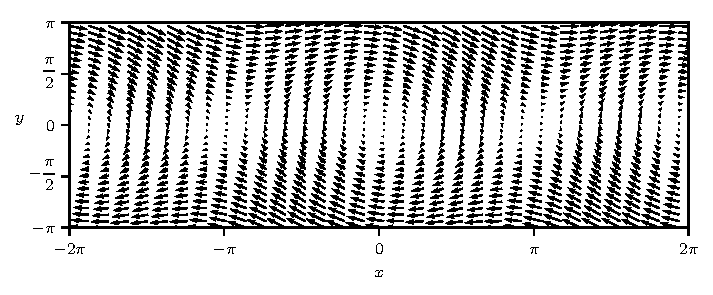
\includegraphics[width=.75\textwidth]{pendulum_phase_plane}

	Plan de phase du pendule simple pour $(k, \omega_0) = (0.1, 1)$.
	\vspace{1cm}
\end{frame}

\begin{frame}[t, c]{Le pendule simple}{Points fixes}
	\begin{itemize}
		\item Il existe certains point du plan de phase pour lesquels le système est en équilibre. Ce sont des \alert{\textbf{points fixes}}. Ils sont donnés par
		\begin{equation}
			\dot{x} = 0 \text{ et } \dot{y} = 0.
			\notag
		\end{equation}

		\bigskip

		\item Pour le pendule simple, ces points fixes sont solutions de
		\begin{equation}
			y = 0 \text{ et } \sin(x) = 0.
			\notag
		\end{equation}
	\end{itemize}

	\vspace{1cm}
\end{frame}

\begin{frame}[t, c]{Le pendule simple}{Points fixes}
	\centering
	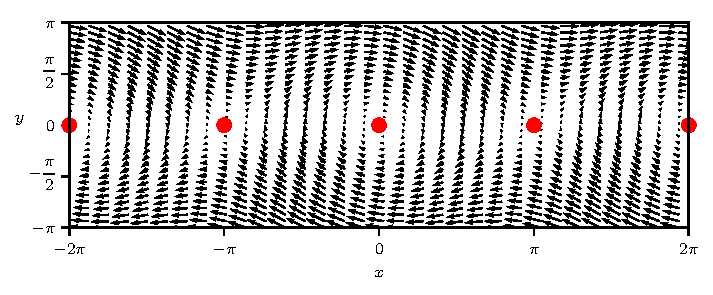
\includegraphics[width=.75\textwidth]{pendulum_fixed_points}

	Plan de phase du pendule simple pour $(k, \omega_0) = (0.1, 1)$.
	\vspace{1cm}
\end{frame}

\begin{frame}[t, c]{Le pendule simple}{Evolution du système}
	\centering
	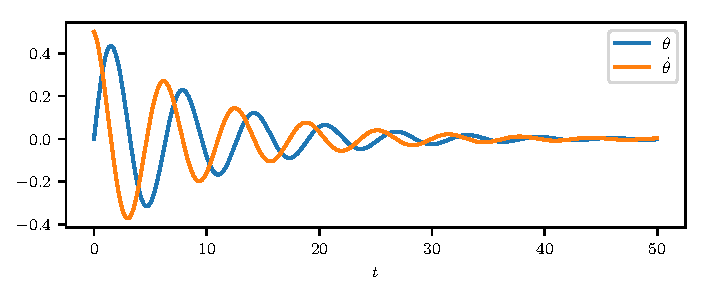
\includegraphics[width=.75\textwidth]{pendulum_fixed_trajectories_0}

	Evolution du pendule simple pour différentes conditions initiales.
	\vspace{1cm}
\end{frame}

\begin{frame}[t, c]{Le pendule simple}{Evolution du système}
	\centering
	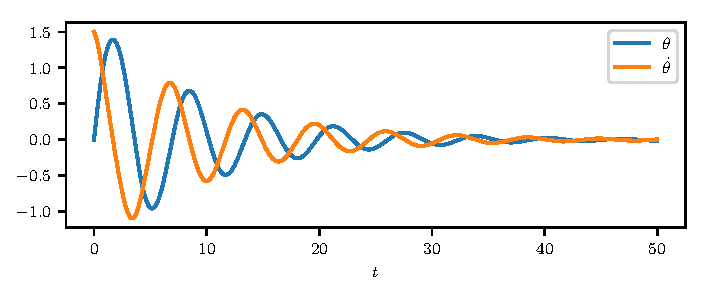
\includegraphics[width=.75\textwidth]{pendulum_fixed_trajectories_2}

	Evolution du pendule simple pour différentes conditions initiales.
	\vspace{1cm}
\end{frame}


\begin{frame}[t, c]{Le pendule simple}{Evolution du système}
	\centering
	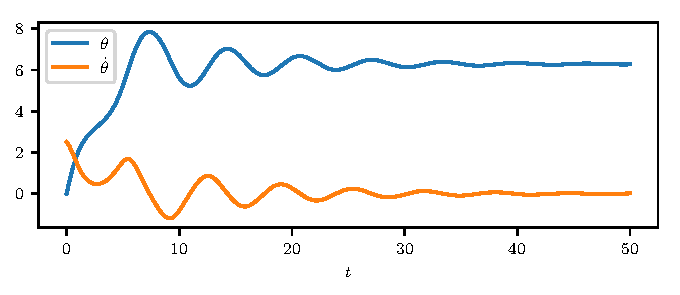
\includegraphics[width=.75\textwidth]{pendulum_fixed_trajectories_4}

	Evolution du pendule simple pour différentes conditions initiales.
	\vspace{1cm}
\end{frame}

\begin{frame}[t, c]{Le pendule simple}{Trajectoires}
	\centering
	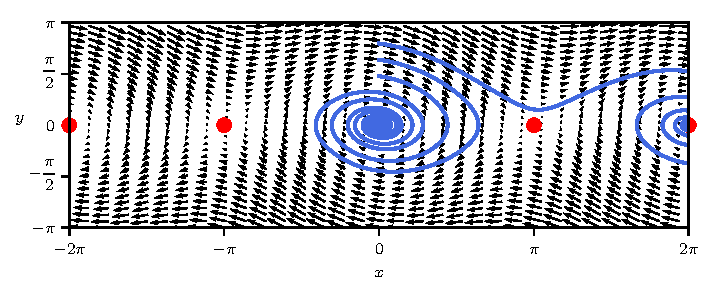
\includegraphics[width=.75\textwidth]{pendulum_fixed_trajectories_bis}

	Plan de phase du pendule simple pour $(k, \omega_0) = (0.1, 1)$.
	\vspace{1cm}
\end{frame}

\begin{frame}[t, c]{Le pendule simple}{Les différents comportements dans l'espace des phases}

	\begin{minipage}{.225\textwidth}
		\centering
		\movie[width=\textwidth, autostart, loop]{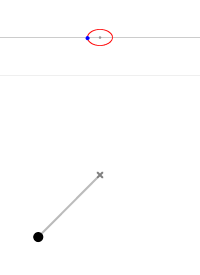
\includegraphics[width=\textwidth]{Pendulum_45deg_0}}{imgs/Pendulum_45deg.mp4}
	\end{minipage}%
	\hfill
	\begin{minipage}{.225\textwidth}
		\centering
		\movie[width=\textwidth, autostart, loop]{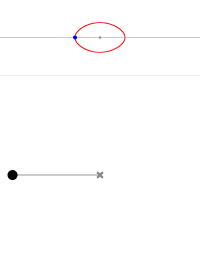
\includegraphics[width=\textwidth]{Pendulum_90deg_0}}{imgs/Pendulum_90deg.mp4}
	\end{minipage}%
	\hfill
	\begin{minipage}{.225\textwidth}
		\movie[width=\textwidth, autostart, loop]{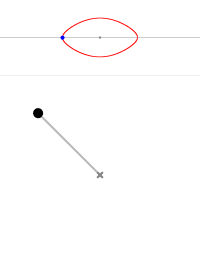
\includegraphics[width=\textwidth]{Pendulum_135deg_0}}{imgs/Pendulum_135deg.mp4}
	\end{minipage}%
	\hfill
	\begin{minipage}{.225\textwidth}
		\movie[width=\textwidth, autostart, loop]{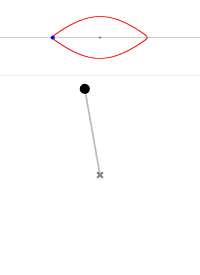
\includegraphics[width=\textwidth]{Pendulum_170deg_0}}{imgs/Pendulum_170deg.mp4}
	\end{minipage}
\end{frame}

\begin{frame}[t, c]{Le pendule simple}{Les différents comportements dans l'espace des phases}

	\centering
	\begin{minipage}{.225\textwidth}
		\centering
		\movie[width=\textwidth, autostart, loop]{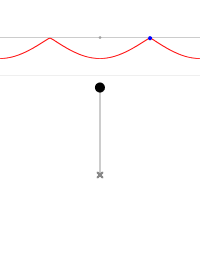
\includegraphics[width=\textwidth]{Pendulum_190deg_0}}{imgs/Pendulum_190deg.mp4}
	\end{minipage}%
	\hspace{1cm}
	\begin{minipage}{.225\textwidth}
		\centering
		\movie[width=\textwidth, autostart, loop]{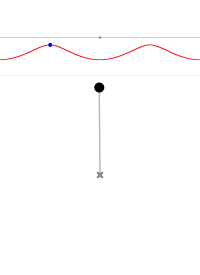
\includegraphics[width=\textwidth]{Pendulum_220deg_0}}{imgs/Pendulum_220deg.mp4}
	\end{minipage}
\end{frame}

\begin{frame}[t, c]{}{}

	\centering

	{\Large \textbf{Illustration}}

	\bigskip

	\textgre{\textbf{Le modèle de Lorenz}}

	\vspace{-2cm}
\end{frame}


\begin{frame}[t, c]{Le modèle de Lorenz}{Un modèle simplifié de convection atmosphérique}

	\begin{itemize}
		\item Le modèle de Lorenz est donné par
		\begin{equation}
			\begin{aligned}
				\dot{x} & = \sigma ( y -x ) \\
				\dot{y} & = x(\rho - z) - y \\
				\dot{z} & = xy - \beta z.
			\end{aligned}
			\notag
		\end{equation}
		Ici, on fixe $\sigma = 10$ et $\beta = \nicefrac{8}{3}$.

		\bigskip

		\item C'est modèle simplifié de convection atmosphérique développé en 1963 par E. Lorenz.
	\end{itemize}

	\vspace{1cm}
\end{frame}

\begin{frame}[t, c]{Le modèle de Lorenz}{Evolution du système pour différents $\rho$}
	\centering
	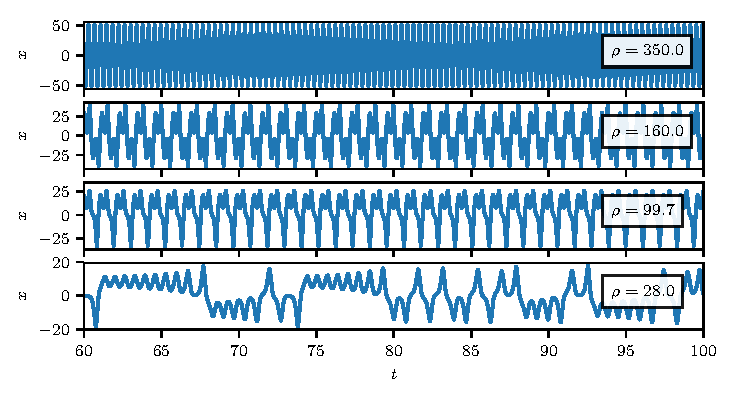
\includegraphics[width=.75\textwidth]{lorenz_time_series}
\end{frame}

\begin{frame}[t, c]{Le modèle de Lorenz}{Portrait de phase}
	\begin{minipage}{.225\textwidth}
		\centering
		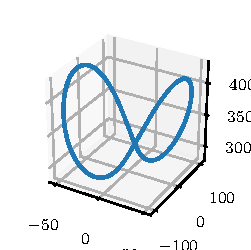
\includegraphics[width=.95\textwidth]{lorenz_phase_plot_0}

		$\rho = 350$
	\end{minipage}%
	\hfill
	\begin{minipage}{.225\textwidth}
		\centering
		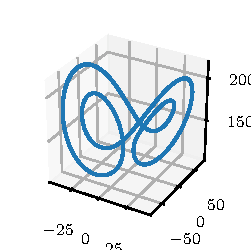
\includegraphics[width=.95\textwidth]{lorenz_phase_plot_1}

		$\rho = 160$
	\end{minipage}%
	\hfill
	\begin{minipage}{.225\textwidth}
		\centering
		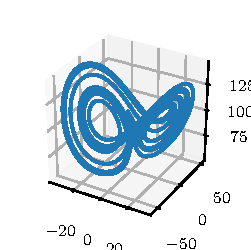
\includegraphics[width=.95\textwidth]{lorenz_phase_plot_2}

		$\rho = 99.7$
	\end{minipage}%
	\hfill
	\begin{minipage}{.225\textwidth}
		\centering
		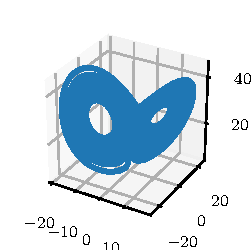
\includegraphics[width=.95\textwidth]{lorenz_phase_plot_3}

		$\rho = 28$
	\end{minipage}

	\vspace{1cm}
\end{frame}

\begin{frame}[t, c]{Le modèle de Lorenz}{Un système chaotique}
	\centering
	\movie[width=.45\textwidth, autostart, loop]{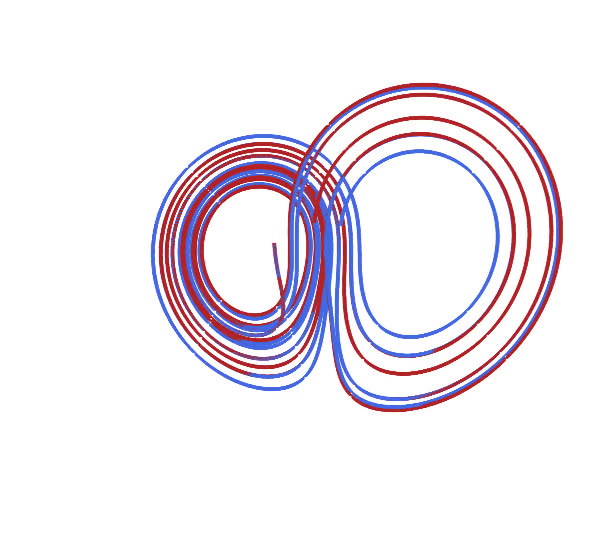
\includegraphics[width=.45\textwidth]{image-316}}{imgs/Lorenz_attractor_JC.mp4}

	\vspace{1cm}
\end{frame}

\begin{frame}[t, c]{}{}

	\centering

	{\Large \textbf{Illustration}}

	\bigskip

	\textgre{\textbf{L'équation logistique}}

	\vspace{-2cm}
\end{frame}

\begin{frame}[t, c]{L'équation logistique}{Un modèle démographique simplifié}

	\begin{itemize}
		\item L'équation logisitque, ou modèle de Verhulst, est donné par
		\begin{equation}
			x_{n+1} = \mu x_n ( 1 - x_n)
			\notag
		\end{equation}
		avec $0 \le x_n \le 1$ et $\mu \in \left[ 0, 4 \right]$.

		\bigskip

		\item Ce modèle en temps discret a été popularisé en 1976 par le biologiste Robert May.
	\end{itemize}

	\vspace{1cm}
\end{frame}

\begin{frame}[t, c]{L'équation logistique}{L'un des routes vers le chaos}
	\centering
	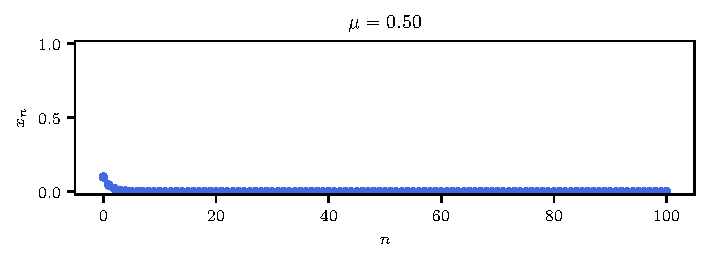
\includegraphics[width=.75\textwidth]{logistic_map_0}
\end{frame}

\begin{frame}[t, c]{L'équation logistique}{L'un des routes vers le chaos}
	\centering
	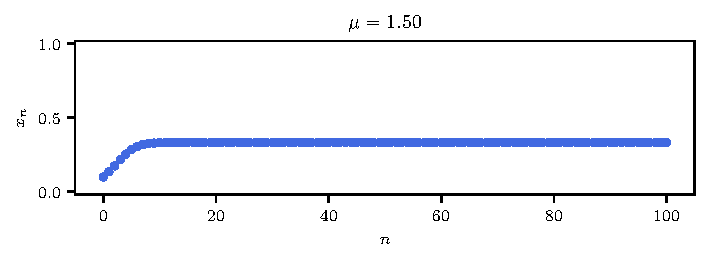
\includegraphics[width=.75\textwidth]{logistic_map_1}
\end{frame}

\begin{frame}[t, c]{L'équation logistique}{L'un des routes vers le chaos}
	\centering
	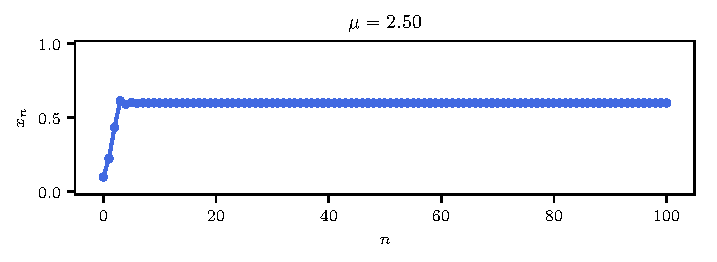
\includegraphics[width=.75\textwidth]{logistic_map_2}
\end{frame}

\begin{frame}[t, c]{L'équation logistique}{L'un des routes vers le chaos}
	\centering
	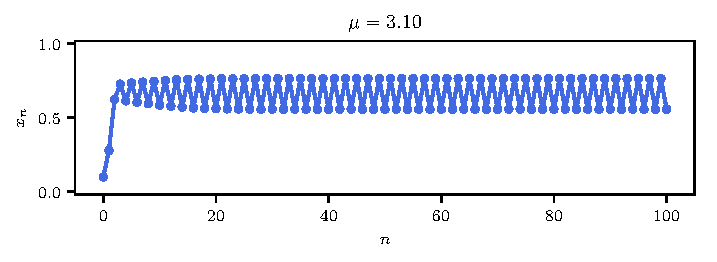
\includegraphics[width=.75\textwidth]{logistic_map_3}
\end{frame}

\begin{frame}[t, c]{L'équation logistique}{L'un des routes vers le chaos}
	\centering
	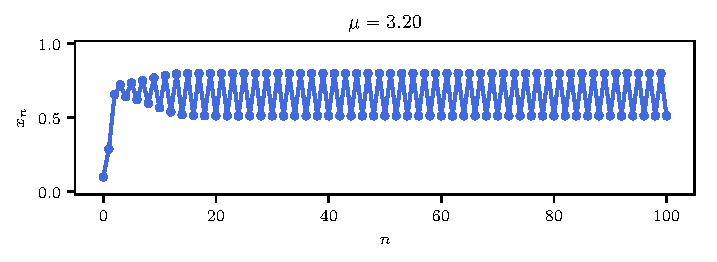
\includegraphics[width=.75\textwidth]{logistic_map_4}
\end{frame}

\begin{frame}[t, c]{L'équation logistique}{L'un des routes vers le chaos}
	\centering
	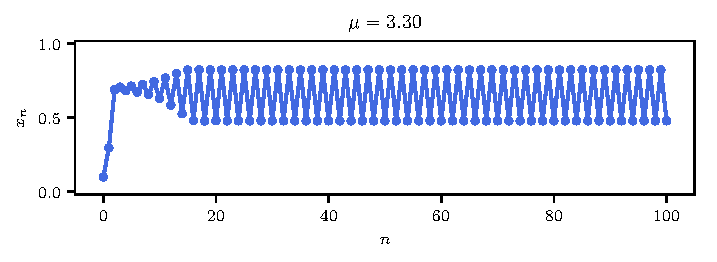
\includegraphics[width=.75\textwidth]{logistic_map_5}
\end{frame}

\begin{frame}[t, c]{L'équation logistique}{L'un des routes vers le chaos}
	\centering
	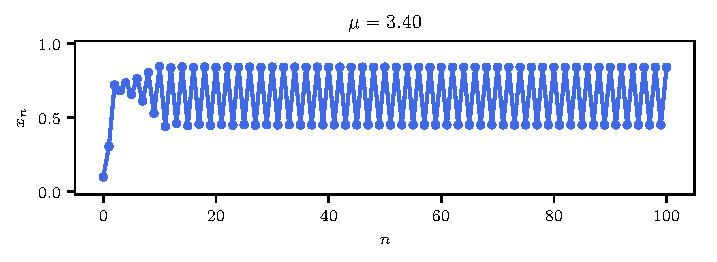
\includegraphics[width=.75\textwidth]{logistic_map_6}
\end{frame}

\begin{frame}[t, c]{L'équation logistique}{L'un des routes vers le chaos}
	\centering
	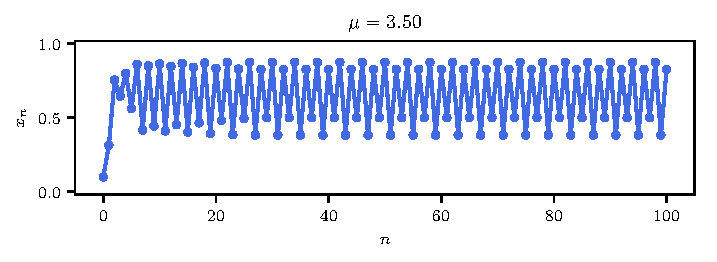
\includegraphics[width=.75\textwidth]{logistic_map_7}
\end{frame}

\begin{frame}[t, c]{L'équation logistique}{L'un des routes vers le chaos}
	\centering
	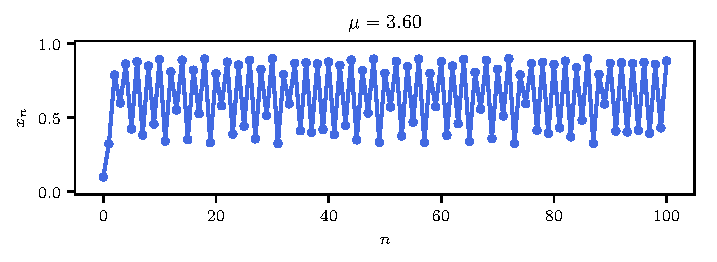
\includegraphics[width=.75\textwidth]{logistic_map_8}
\end{frame}

\begin{frame}[t, c]{L'équation logistique}{L'un des routes vers le chaos}
	\centering
	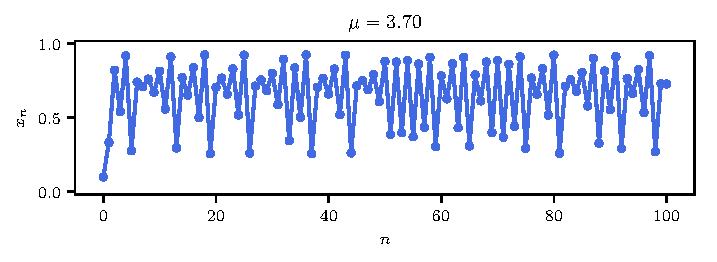
\includegraphics[width=.75\textwidth]{logistic_map_9}
\end{frame}

\begin{frame}[t, c]{L'équation logistique}{L'un des routes vers le chaos}
	\centering
	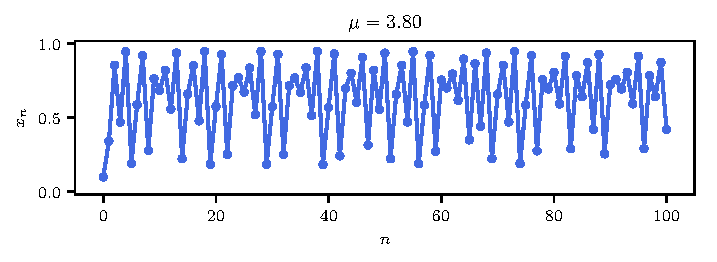
\includegraphics[width=.75\textwidth]{logistic_map_10}
\end{frame}

\begin{frame}[t, c]{L'équation logistique}{L'un des routes vers le chaos}
	\centering
	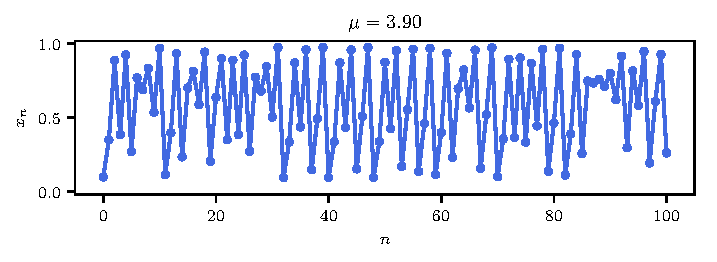
\includegraphics[width=.75\textwidth]{logistic_map_11}
\end{frame}

\begin{frame}[t, c]{L'équation logistique}{Diagramme de bifurcation}
	\centering
	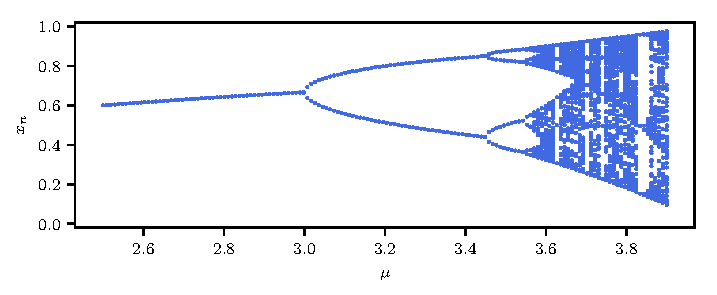
\includegraphics[width=.75\textwidth]{logistic_map_bifurcation}
\end{frame}

\end{document}
